\documentclass{article}
\usepackage{graphicx} %package to manage images
\graphicspath{ {./figures/} }
\usepackage{hyperref}
\usepackage{caption}
\usepackage[font=scriptsize]{subcaption}
\captionsetup[figure]{labelsep=none}
\captionsetup[table]{labelsep=none}
\usepackage{bbm}
\usepackage{amsmath}
\usepackage{import}
\usepackage{array}
\usepackage{booktabs}
\usepackage{afterpage}
\usepackage{floatrow}
\usepackage{pdflscape}
\usepackage{soul}
\usepackage{float}
\usepackage{adjustbox}
\usepackage{longtable}

\begin{document}

\maketitle

% \section{underweight: kitagawa decomposition}

% using wealth in reweighting instead of parity

% \begin{table}[H]
%     \centering
%     \footnotesize % shrink text
%     \caption{: Dalit fwd decomposition}
%     \label{tab:sumstat}
%     \adjustbox{width=\textwidth}{\begin{tabular}{l*{6}{c}}
\toprule
            &\multicolumn{1}{c}{Wealth 1st Q}&\multicolumn{1}{c}{Wealth 2nd Q}&\multicolumn{1}{c}{Wealth 3rd Q}&\multicolumn{1}{c}{Wealth 4th Q}&\multicolumn{1}{c}{Total}&\multicolumn{1}{c}{Percent}\\
\midrule
\midrule
Prop. pregnant women (Fwd)&        0.11&        0.17&        0.27&        0.44&            &            \\
Avg pre-pregnancy underweight (Fwd)&       25.40&       23.42&       15.24&       11.06&       15.97&            \\
Prop. pregnant women (Dalit)&        0.34&        0.26&        0.24&        0.16&            &            \\
Avg pre-pregnancy underweight (Dalit)&       29.28&       22.28&       19.24&       13.04&       22.41&            \\
Difference in underweight (Dalit-Forward)&        3.88&       -1.14&        3.99&        1.98&        6.45&            \\
Within parity difference (rate)&        0.88&       -0.24&        1.02&        0.60&        2.26&       34.99\\
Between parity difference (compositional)&        6.15&        1.96&       -0.59&       -3.33&        4.19&       65.01\\
\bottomrule
\end{tabular}
}
% \end{table}

% \begin{table}[H]
%     \centering
%     \footnotesize % shrink text
%     \caption{: Adivasi fwd decomposition}
%     \label{tab:sumstat}
%     \adjustbox{width=\textwidth}{\begin{tabular}{l*{6}{c}}
\toprule
            &\multicolumn{1}{c}{Wealth 1st Q}&\multicolumn{1}{c}{Wealth 2nd Q}&\multicolumn{1}{c}{Wealth 3rd Q}&\multicolumn{1}{c}{Wealth 4th Q}&\multicolumn{1}{c}{Total}&\multicolumn{1}{c}{Percent}\\
\midrule
\midrule
Prop. pregnant women (Fwd)&        0.11&        0.17&        0.27&        0.44&            &            \\
Avg pre-pregnancy underweight (Fwd)&       27.24&       23.80&       15.34&       11.01&       16.24&            \\
Prop. pregnant women (Adivasi)&        0.50&        0.25&        0.16&        0.09&            &            \\
Avg pre-pregnancy underweight (Adivasi)&       30.61&       27.54&       20.37&       10.81&       26.34&            \\
Difference in underweight (Adivasi-Forward)&        3.37&        3.73&        5.03&       -0.19&       10.10&            \\
Within parity difference (rate)&        1.03&        0.78&        1.09&       -0.05&        2.86&       28.29\\
Between parity difference (compositional)&       11.11&        1.91&       -2.00&       -3.78&        7.24&       71.71\\
\bottomrule
\end{tabular}
}
% \end{table}



% \begin{table}[H]
%     \centering
%     \footnotesize % shrink text
%     \caption{: Muslim fwd decomposition}
%     \label{tab:sumstat}
%     \adjustbox{width=\textwidth}{\begin{tabular}{l*{6}{c}}
\toprule
            &\multicolumn{1}{c}{Wealth 1st Q}&\multicolumn{1}{c}{Wealth 2nd Q}&\multicolumn{1}{c}{Wealth 3rd Q}&\multicolumn{1}{c}{Wealth 4th Q}&\multicolumn{1}{c}{Total}&\multicolumn{1}{c}{Percent}\\
\midrule
\midrule
Prop. preg (Fwd)&        0.11&        0.17&        0.27&        0.44&            &            \\
Avg pre-preg underweight (Fwd)&       25.47&       23.29&       13.97&       10.92&       15.54&            \\
Prop. preg (Muslim)&        0.26&        0.23&        0.25&        0.27&            &            \\
Avg pre-preg underweight (Muslim)&       20.39&       15.20&       11.96&        8.87&       14.05&            \\
Difference in underweight (Muslim-Forward)&       -5.08&       -8.09&       -2.01&       -2.05&       -1.49&            \\
Within group difference&       -0.95&       -1.61&       -0.52&       -0.73&       -3.81&      255.69\\
Between group difference&        3.33&        1.03&       -0.33&       -1.72&        2.32&     -155.69\\
\bottomrule
\end{tabular}
}
% \end{table}

% \begin{table}[H]
%     \centering
%     \footnotesize % shrink text
%     \caption{: OBC fwd decomposition}
%     \label{tab:sumstat}
%     \adjustbox{width=\textwidth}{\begin{tabular}{l*{6}{c}}
\toprule
            &\multicolumn{1}{c}{mtitles1}&\multicolumn{1}{c}{wealth2}&\multicolumn{1}{c}{wealth3}&\multicolumn{1}{c}{wealth4}&\multicolumn{1}{c}{total}&\multicolumn{1}{c}{pct}\\
\midrule
\midrule
Prop. preg (Fwd)&        0.11&        0.17&        0.27&        0.44&            &            \\
Avg pre-preg underweight (Fwd)&       25.47&       23.29&       13.97&       10.92&       15.54&            \\
Prop. preg (OBC)&        0.22&        0.25&        0.26&        0.27&            &            \\
Avg pre-preg underweight (OBC)&       29.88&       23.91&       18.35&       11.64&       20.45&            \\
Difference in underweight (OBC-Forward)&        4.41&        0.62&        4.38&        0.72&        4.91&            \\
Within group difference&        0.74&        0.13&        1.17&        0.26&        2.29&       46.74\\
Between group difference&        3.01&        1.72&       -0.22&       -1.90&        2.61&       53.26\\
\bottomrule
\end{tabular}
}
% \end{table}




\begin{figure}[H]
    \centering
    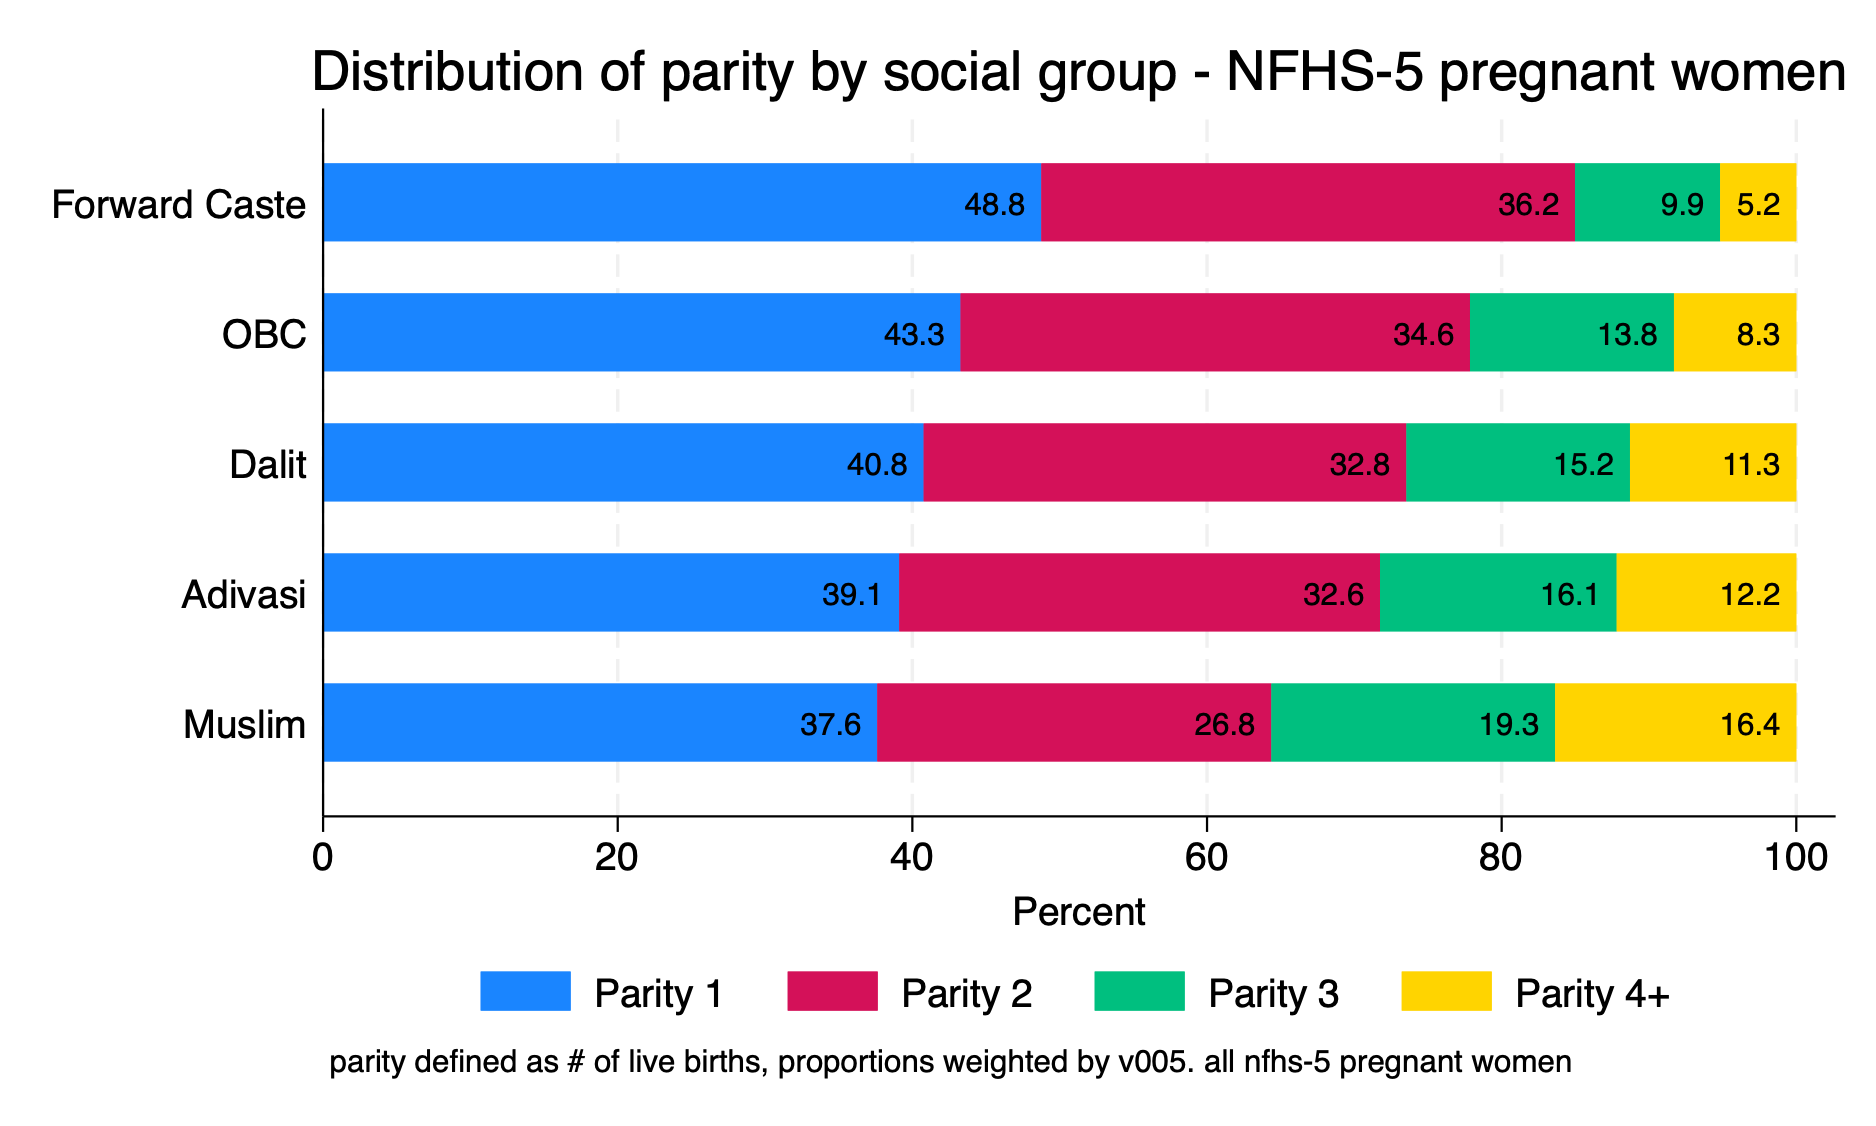
\includegraphics[width=\textwidth]{figures/parity distribution of pregnant women by social group.png}
\end{figure}

\begin{figure}[H]
    \centering
    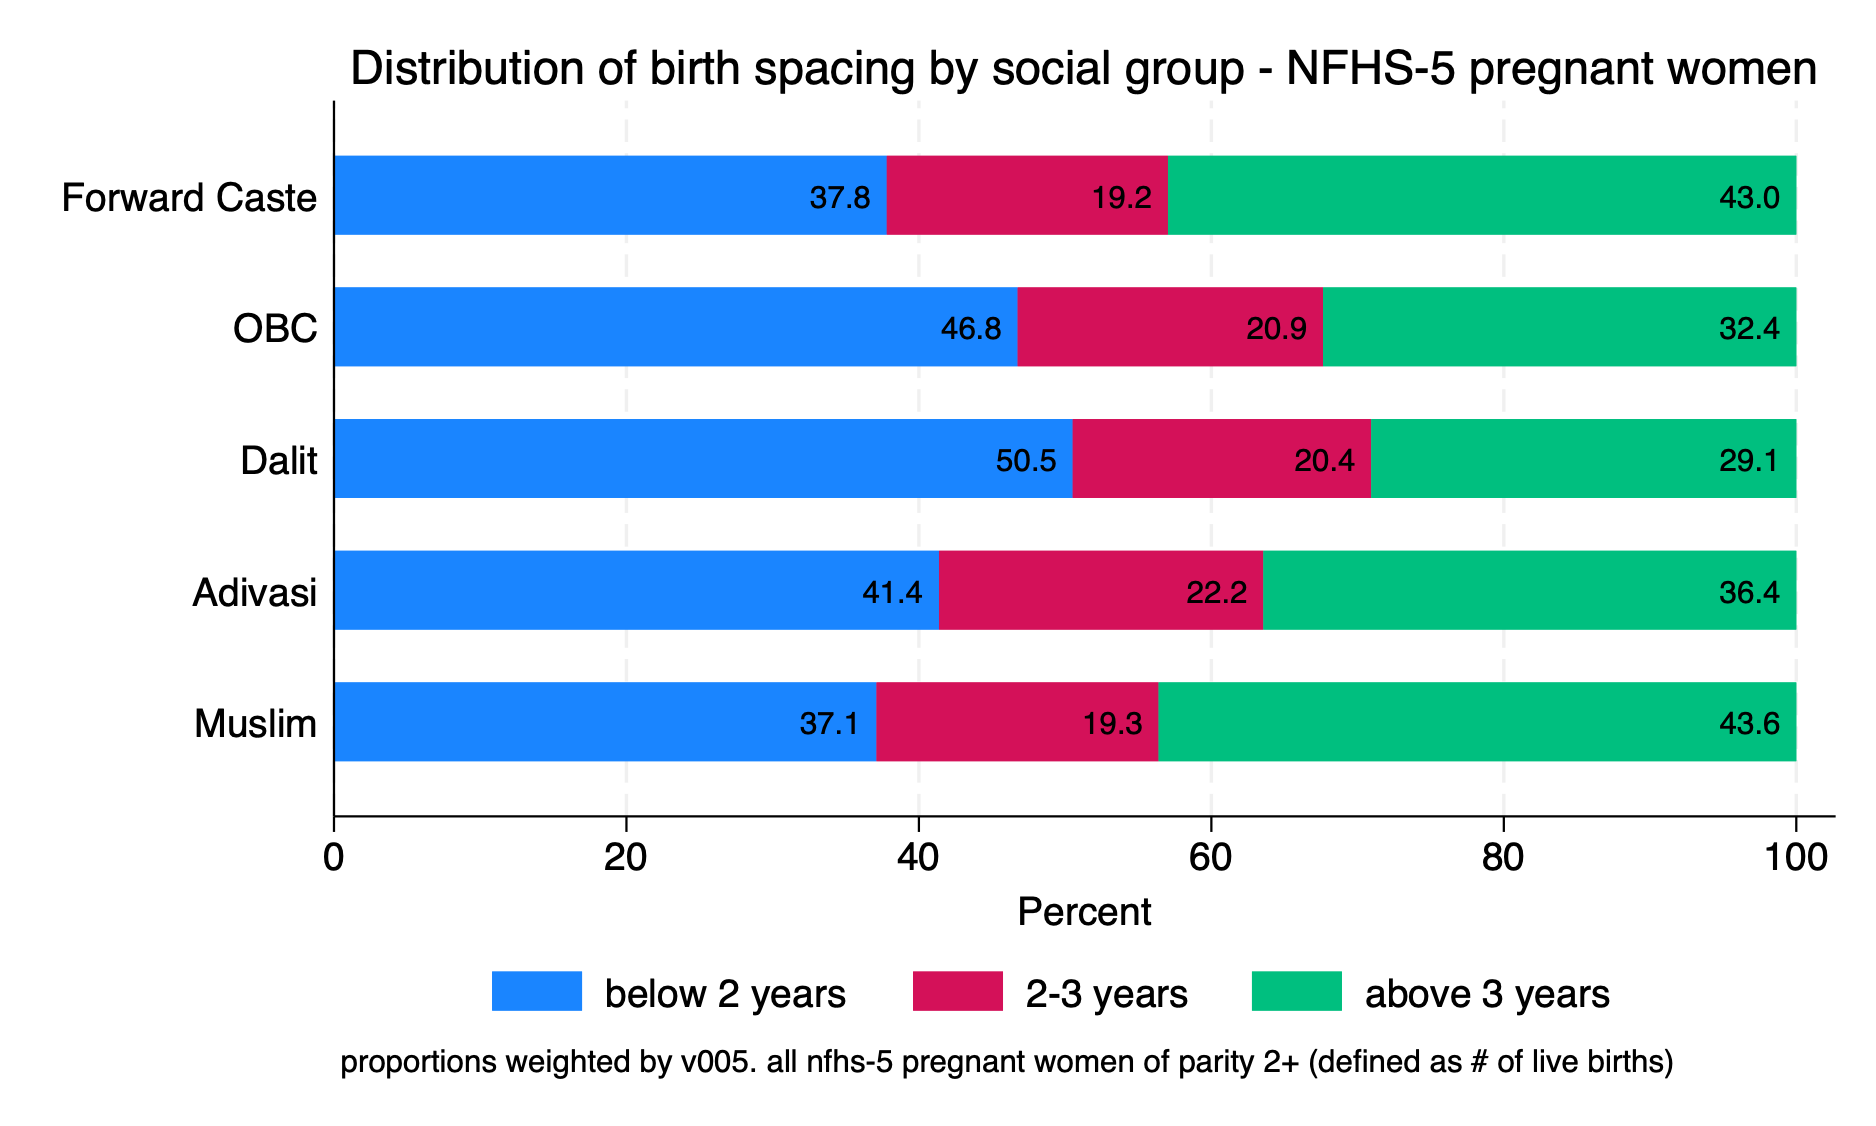
\includegraphics[width=\textwidth]{figures/birth spacing distribution of pregnant women by social group.png}
\end{figure}

\newpage
\begin{figure}[H]
    \centering
    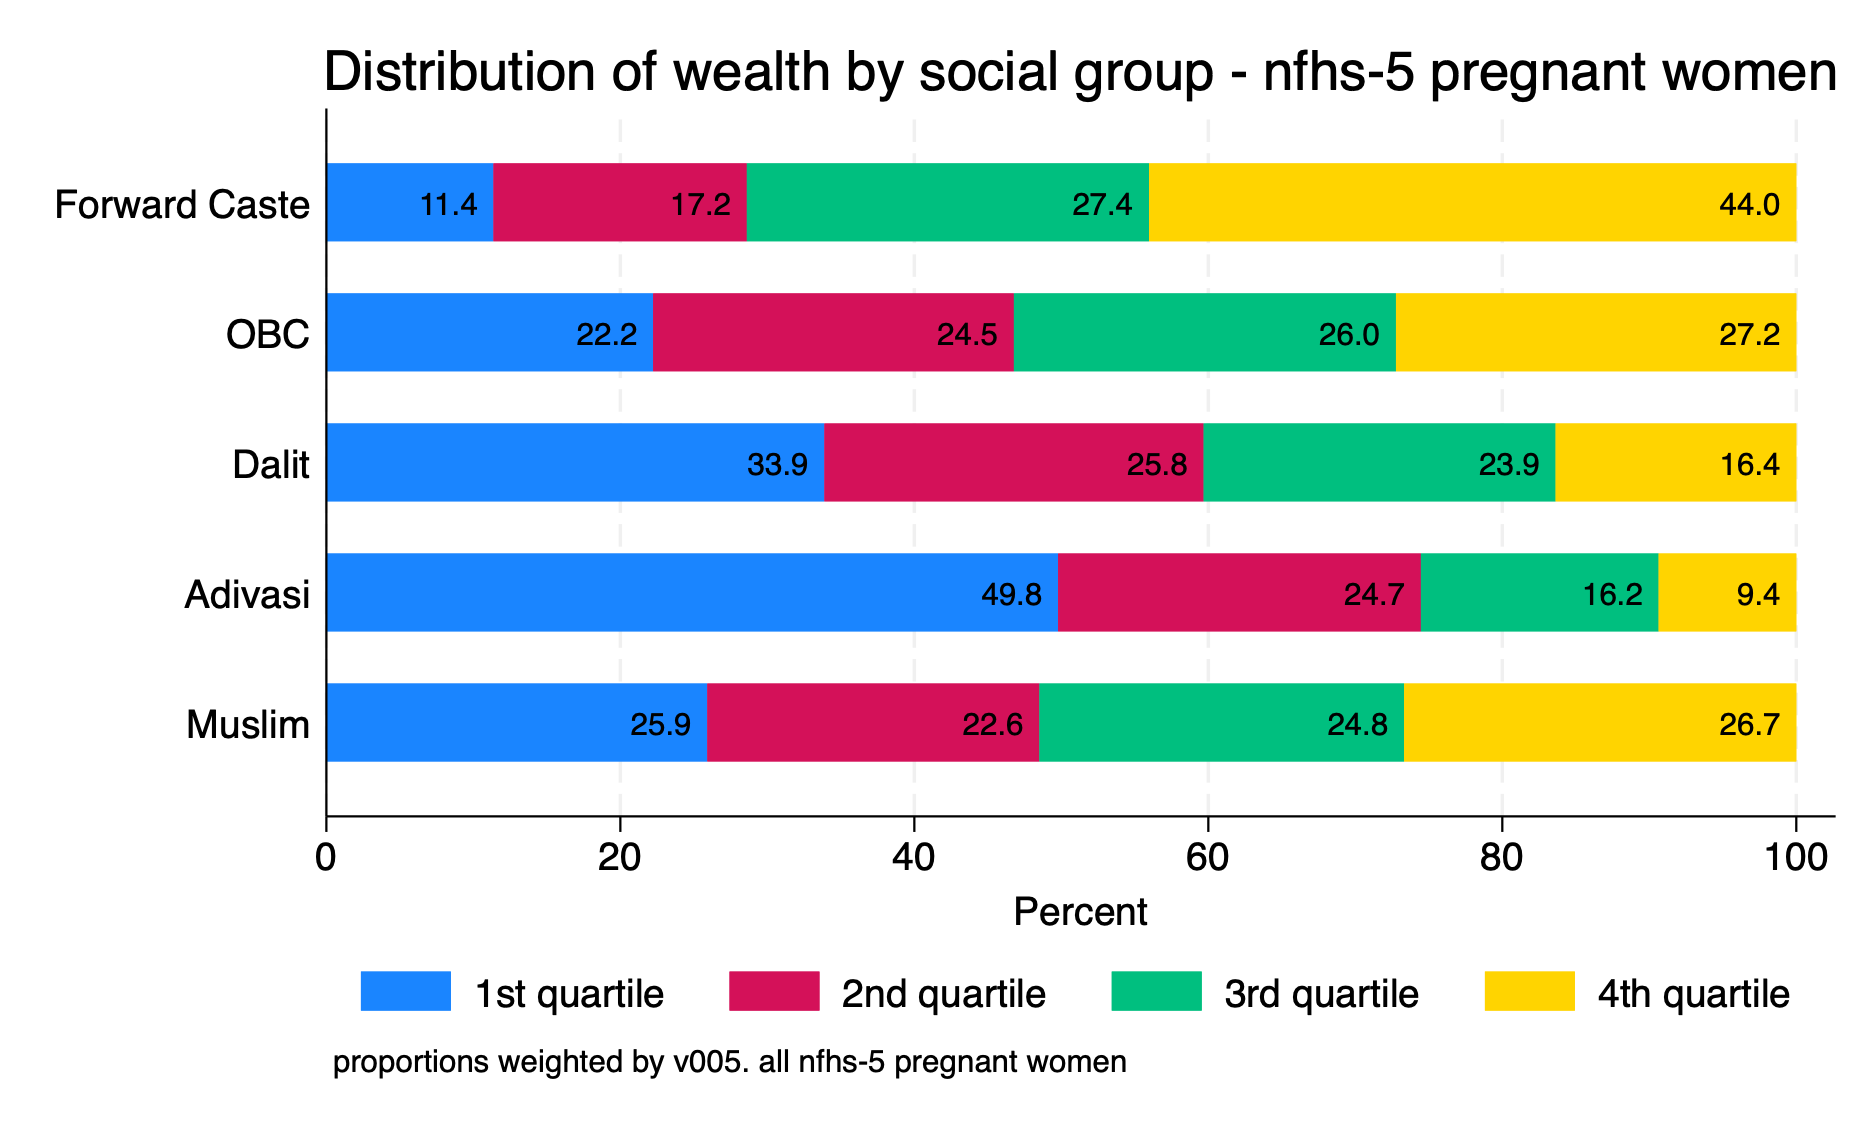
\includegraphics[width=\textwidth]{figures/wealth distribution of pregnant women by social group.png}
\end{figure}






\end{document}


